%%
%% getstart.tex -- Flight Gear documentation: The FlightGear Manual
%% Chapter file
%%
%% Written by Michael Basler, started September 1998.
%%
%% Copyright (C) 2002 Michael Basler
%%
%%
%% This program is free software; you can redistribute it and/or
%% modify it under the terms of the GNU General Public License as
%% published by the Free Software Foundation; either version 2 of the
%% License, or (at your option) any later version.
%%
%% This program is distributed in the hope that it will be useful, but
%% WITHOUT ANY WARRANTY; without even the implied warranty of
%% MERCHANTABILITY or FITNESS FOR A PARTICULAR PURPOSE.  See the GNU
%% General Public License for more details.
%%
%% You should have received a copy of the GNU General Public License
%% along with this program; if not, write to the Free Software
%% Foundation, Inc., 675 Mass Ave, Cambridge, MA 02139, USA.
%%
%% $Id: flight.tex,v 0.5 0.6 2002/09/09 michael
%% (Log is kept at end of this file)

%%%%%%%%%%%%%%%%%%%%%%%%%%%%%%%%%%%%%%%%%%%%%%%%%%%%%%%%%%%%%%%%%%%%%%%%%%%%%%%%
%%%%%%%%%%%%%%%
\chapter{In-flight: All about instruments, keystrokes and menus}
\label{flight}
%%%%%%%%%%%%%%%%%%%%%%%%%%%%%%%%%%%%%%%%%%%%%%%%%%%%%%%%%%%%%%%%%%%%%%%%%%%%%%%%
%%%%%%%%%%%%%%%
\markboth{\thechapter.\hspace*{1mm} FLIGHT}{\thesection\hspace*{1mm} KEYBOARD
CONTROLS}

The following is a description of the main systems for controlling the
program and piloting the plane. It is assumed that the reader is already 
familiar with flying, possibly from experience on other simulators. If you are
completely new to flying, the tutorials in section \ref{tutorials} are a better
resource for learning to fly using FlightGear{}.

A short leaflet showing the standard keys and designed to be printed can be found at
\medskip
\web{http://www.flightgear.org/Docs/FGShortRef.pdf}.
\medskip

\noindent
A reference to most of the keyboard controls can be found under the Help menu in the simulator.

%%%%%%%%%%%%%%%%%%%%%%%%%%%%%%%%%%%%%%%%%%%%%%%%%%%%%%%%%%%%%%%%%%%%%%%%%%%%%%%%
%%%%%%%%%%%%%%%
\section{Starting the engine}\index{engine!starting}
%%%%%%%%%%%%%%%%%%%%%%%%%%%%%%%%%%%%%%%%%%%%%%%%%%%%%%%%%%%%%%%%%%%%%%%%%%%%%%%%
%%%%%%%%%%%%%%%

Depending on the type of aircraft, you may have to start the engine(s) before you can
go flying. The instructions below are generic. Check the aircraft help or aircraft tutorials
for more specific instructions.

Once you've started the engine, you should check whether the \Index{parking brake}s are engaged.
If so, press the `B' to release them.

\subsection{Piston Aircraft}\index{engine!starting!piston}

For piston-engined aircraft, the magnetos are controlled by the `\{' and `\}' keys. On most aircraft, the starter is engaged using the `s' key. On multi-engined aircraft you can select which engines to control. Use `\~' to select all the engines at once. Most magnetos have 4 positions -
OFF, LEFT, RIGHT and BOTH. So, to start the selected engine, press the `\}' key three times, then hold down `s'.

Note that the starting procedure for powerful WWII-era fighter aircraft is often more complex. See the aircraft help for details.

\subsection{Turboprop Aircraft}\index{engine!starting!turboprop}

Starting a turbo-prop engine generally requires simply moving the condition lever from Off to Idle, using 'm'.

\subsection{Jet Aircraft}\index{engine!starting!jet}

Starting a jet aircraft is significantly more complex, and the controls vary between different aircraft.

\begin{enumerate}
\item Set cutoff ON
\item Engage the starter
\item Once the engines spools up to approximately 5\% N1, set cutoff OFF
\item Disengage the starter once the engine has reached operational speed.
\end{enumerate}

%%%%%%%%%%%%%%%%%%%%%%%%%%%%%%%%%%%%%%%%%%%%%%%%%%%%%%%%%%%%%%%%%%%%%%%%%%%%%%%%
%%%%%%%%%%%%%%%
\section{Keyboard controls}\index{keyboard controls}
%%%%%%%%%%%%%%%%%%%%%%%%%%%%%%%%%%%%%%%%%%%%%%%%%%%%%%%%%%%%%%%%%%%%%%%%%%%%%%%%
%%%%%%%%%%%%%%%

While \Index{joystick}s, \Index{yoke}s and \Index{rudder pedals} are supported,
you can fly \FlightGear{} using the keyboard alone or in conjunction with a mouse,
described below.

However you control the aircraft, you will need to use the keyboard for at least some controls.

These key bindings\index{keybindings!configuration} are not hard-coded, but
user-adjustable. You can check and change these setting via the file
\texttt{keyboard.xml}\index{keyboard.xml} which can be found in the main
\FlightGear{} directory. This is a human-readable plain ASCII file.
Although it's perhaps not the best idea for beginners to modify this file,
more advanced users will find it useful to change key bindings according to
their wished, e.g. to match other simulators.

\subsection{Aircraft controls}\index{keyboard controls!aircraft}

In order to have full control of the plane during flight via the keyboard you should ensure that
\texttt{\Index{NumLock}} is on, and the \FlightGear{} window is in focus.

\medskip
\centerline{%%
%% tab2.tex -- Flight Gear documentation: The FlightGear Manual
%% Keyboard controls table 1/Main controls
%%
%% Written by Michael Basler, started September 1998.
%%
%% Copyright (C) 2002 Michael Basler
%%
%%
%% This program is free software; you can redistribute it and/or
%% modify it under the terms of the GNU General Public License as
%% published by the Free Software Foundation; either version 2 of the
%% License, or (at your option) any later version.
%%
%% This program is distributed in the hope that it will be useful, but
%% WITHOUT ANY WARRANTY; without even the implied warranty of
%% MERCHANTABILITY or FITNESS FOR A PARTICULAR PURPOSE.  See the GNU
%% General Public License for more details.
%%
%% You should have received a copy of the GNU General Public License
%% along with this program; if not, write to the Free Software
%% Foundation, Inc., 675 Mass Ave, Cambridge, MA 02139, USA.
%%
%% $Id: tab1.tex,v 0.6 2002/09/09 michael
%% (Log is kept at end of this file)
%%%%%%%%%%%%%%%%%%%%%%%%%%%%%%%%%%%%%%%%%%%%%%%%%%%%%%%%%%%%%%%%%%%%%%%%%%%%%%%%%%%%%%%%%%%%%%%%
\begin{tabular}{|l|l|}\hline
\IfLanguageName{english}{
  Key      &  Action\\\hline
 9 / 3     &  Throttle\index{throttle}\\
 4 / 6     &  Aileron\index{aileron}\\
 8 / 2     &  Elevator\index{elevator}\\
 0 / Enter &  Rudder\index{rudder}\\
 5         &  Center aileron/elevator/rudder\\
 7 / 1     &  Elevator \Index{trim}\\\hline
}{}
\IfLanguageName{french}{
  Touche      &  Action\\\hline
 9 / 3     &  Commande des gaz\index{gaz}\\
 4 / 6     &  Aileron\index{aileron}\\
 8 / 2     &  Gouverne de profondeur\index{gouverne de profondeur}\\
 0 / Entr\'{e}e &  gouverne de direction\index{gouverne de direction}\\
 5         &  Centrage des ailerons/gouverne de profondeur/direction\\
 7 / 1     &  Trim de la gouverne de profondeur \Index{trim}\\\hline
}{}
\IfLanguageName{italian}{
  Pulsante/i      &  Azione\\\hline
 9 / 3     &  Manetta (Throttle)\index{manetta}\index{throttle}\\
 4 / 6     &  Alettoni\index{Alettoni}\\
 8 / 2     &  Elevatore (timone di coda)\index{Elevatore}\\
 0 / Invio &  Timone di direzione\index{gouverne de direction}\\
 5         &  Centra alettoni, timone di coda e di direzione\\
 7 / 1     &  Regola il trim \Index{trim}\\\hline
}{}

\end{tabular}

%% revision 0.5 2002/02/15 michael
%% Initial revision
}
Tab.\,1: \textit{Main aircraft controls.}
\medskip

The following keys control the engines \index{engine controls}:

\medskip
\centerline{%%
%% tab7.tex -- Flight Gear documentation: The FlightGear Manual
%% Keyboard controls table 6/Engine related controls
%%
%% Written by Michael Basler, started September 1998.
%%
%% Copyright (C) 2002 Michael Basler
%%
%%
%% This program is free software; you can redistribute it and/or
%% modify it under the terms of the GNU General Public License as
%% published by the Free Software Foundation; either version 2 of the
%% License, or (at your option) any later version.
%%
%% This program is distributed in the hope that it will be useful, but
%% WITHOUT ANY WARRANTY; without even the implied warranty of
%% MERCHANTABILITY or FITNESS FOR A PARTICULAR PURPOSE.  See the GNU
%% General Public License for more details.
%%
%% You should have received a copy of the GNU General Public License
%% along with this program; if not, write to the Free Software
%% Foundation, Inc., 675 Mass Ave, Cambridge, MA 02139, USA.
%%
%% $Id: tab6.tex,v 0.6 2002/09/09 michael
%% (Log is kept at end of this file)
%%%%%%%%%%%%%%%%%%%%%%%%%%%%%%%%%%%%%%%%%%%%%%%%%%%%%%%%%%%%%%%%%%%%%%%%%%%%%%%%%%%%%%%%%%%%%%%%
\begin{tabular}{|l|l|}\hline
  \ifchinese
  按键   &    操作\\\hline
  !     &    选择第一号发动机\\
  @     &    选择第二号发动机\\
  \#    &    选择第三号发动机\\
  \$    &    选择第四号发动机\\
  $\sim$$ &  选择所有发动机\\\hline
  \{    &    减少所选发动机的磁电机档位\\
  \}    &    增加所选发动机的磁电机档位\\
  s     &    为所选的发动机点火启动\\
  M / m &    贫油/富油所选发动机的油气混合比\\
  N / n &    减少/增加所选发动机的螺旋桨转速 \\\hline
  \fi
\iffalse
\IfLanguageName{english}{
Key      &  Action\\ \hline
   !     & Select 1st engine\\
   @	   & Select 2nd engine\\
  \#     & Select 3rd engine\\
  \$     & Select 4th engine\\
  $\sim$ & Select all engines\\\hline
  \{     & Decrease magneto on selected engine\\
  \}     & Increase magneto on selected engine\\
   s     & Fire starter on selected engine(s)\\
  M / m  & Lean/Enrich selected engine mixture\\
  N / n  & Decrease/Increase selected propeller RPM\\\hline
}{}
\fi
\IfLanguageName{french}{
Touche     &  Action\\ \hline
   !     & S\'{e}l\'{e}ctionne le premier moteur\\
   @	 & S\'{e}l\'{e}ctionne le deuxi\`{e}me moteur\\
  \#     & S\'{e}l\'{e}ctionne le troisi\`{e}me moteur\\
  \$     & S\'{e}l\'{e}ctionne le quatri\`{e}me moteur\\
  $\sim$ & S\'{e}l\'{e}ctionne tous les moteurs\\\hline
  \{     & D\'{e}cr\'{e}mente le magn\'{e}to sur le moteur s\'{e}lectionn\'{e}\\
  \}     & Incr\'{e}mente le magn\'{e}to sur le moteur s\'{e}lectionn\'{e}\\
   s     & D\'{e}marrage du/des moteur(s) s\'{e}lectionn\'{e}(s)\\
  M / m  & Appauvrir/Enrichir le m\'{e}lange du moteur s\'{e}lectionn\'{e}\\
  N / n  & Diminue/Augmente le nombre de tours par minute du moteur s\'{e}lectionn\'{e}\\\hline
}{}
\IfLanguageName{italian}{
Pulsante/i &  Azione\\ \hline
   !     & Seleziona il 1\textdegree{} motore\\
   @	   & Seleziona il 2\textdegree{} motore\\
  \#     & Seleziona il 3\textdegree{} motore\\
  \$     & Seleziona il 4\textdegree{} motore\\
  $\sim$ & Seleziona tutti i motori\\\hline
  \{     & Diminuisce la forza dei magneti sui motori selezionati\\
  \}     & Aumenta la forza dei magneti sui motori selezionati\\
   s     & Avvia i(l) motore/i selezionato/i\\
  M / m  & Impoverisce/Arricchisce la miscela del motore selezionato\\
  N / n  & Diminuisce/Aumenta il passo dell'elica del motore selezionato\\\hline
}{}
\end{tabular}

%% revision 0.5 2002/02/15 michael
%% Initial revision
}
Tab.\,2: \textit{Engine control keys}
\medskip

\subsection{Simulator controls}\index{keyboard controls!simulator controls}

To change the \Index{view direction}, you must de-activate \texttt{NumLock}. The available controls are as follows:
\medskip

\centerline{%%
%% tab3.tex -- Flight Gear documentation: The FlightGear Manual
%% Keyboard controls table 2/View directions
%%
%% Written by Michael Basler, started September 1998.
%%
%% Copyright (C) 2002 Michael Basler
%%
%%
%% This program is free software; you can redistribute it and/or
%% modify it under the terms of the GNU General Public License as
%% published by the Free Software Foundation; either version 2 of the
%% License, or (at your option) any later version.
%%
%% This program is distributed in the hope that it will be useful, but
%% WITHOUT ANY WARRANTY; without even the implied warranty of
%% MERCHANTABILITY or FITNESS FOR A PARTICULAR PURPOSE.  See the GNU
%% General Public License for more details.
%%
%% You should have received a copy of the GNU General Public License
%% along with this program; if not, write to the Free Software
%% Foundation, Inc., 675 Mass Ave, Cambridge, MA 02139, USA.
%%
%% $Id: tab2.tex,v 0.6 2002/09/09 michael
%% (Log is kept at end of this file)
%%%%%%%%%%%%%%%%%%%%%%%%%%%%%%%%%%%%%%%%%%%%%%%%%%%%%%%%%%%%%%%%%%%%%%%%%%%%%%%%%%%%%%%%%%%%%%%%
\begin{tabular}{|c|l|}\hline
\iflanguage{english}{
   Numpad Key  &  View direction\index{view directions}\\\hline
    Shift-8  & Forward\\
    Shift-7  & Left/forward\\
    Shift-4  & Left\\
    Shift-1  & Left/back\\
    Shift-2  & Back\\
    Shift-3  & Right/back\\
    Shift-6  & Right\\
    Shift-9  & Right/forward\\\hline
}{}
\iflanguage{french}{
   Touche pav\'{e} num\'{e}rique & Angle de vue\index{angle de vue}\\\hline
    Shift-8  & Vers l'avant\\
    Shift-7  & Avant/Gauche\\
    Shift-4  & Gauche\\
    Shift-1  & Arri\`{e}re/Gauche\\
    Shift-2  & Arri\`{e}re\\
    Shift-3  & Arri\`{e}re/Droit\\
    Shift-6  & Droit\\
    Shift-9  & Avant/Droit\\\hline
}{}
\end{tabular}

%% revision 0.5 2002/02/15 michael
%% Initial revision
}
Tab.\,3: \textit{View directions}
\medskip

Additionally, the following keys allow you to change the view:
\medskip

\noindent
\centerline{%%
%% tab4.tex -- Flight Gear documentation: Installation and Getting Started
%% Keyboard controls table 3/Additional view options
%%
%% Written by Michael Basler, started September 1998.
%%
%% Copyright (C) 2002 Michael Basler (pmb@epost.de)
%%
%%
%% This program is free software; you can redistribute it and/or
%% modify it under the terms of the GNU General Public License as
%% published by the Free Software Foundation; either version 2 of the
%% License, or (at your option) any later version.
%%
%% This program is distributed in the hope that it will be useful, but
%% WITHOUT ANY WARRANTY; without even the implied warranty of
%% MERCHANTABILITY or FITNESS FOR A PARTICULAR PURPOSE.  See the GNU
%% General Public License for more details.
%%
%% You should have received a copy of the GNU General Public License
%% along with this program; if not, write to the Free Software
%% Foundation, Inc., 675 Mass Ave, Cambridge, MA 02139, USA.
%%
%% $Id: tab3.tex,v 0.6 2002/09/09 michael
%% (Log is kept at end of this file)
%%%%%%%%%%%%%%%%%%%%%%%%%%%%%%%%%%%%%%%%%%%%%%%%%%%%%%%%%%%%%%%%%%%%%%%%%%%%%%%%%%%%%%%%%%%%%%%%
\begin{tabular}{|l|l|}\hline
 Key              &         Action\\\hline
 P                &    Toggle \Index{instrument panel} on/off \\
 c                &    Toggle3D/2D cockpit
 											 \index{2D cockpit} (if both are available)
 											 \index{3D cockpit}\index{cockpit}\\
 s                &    Cycle panel style full/mini\\
 Shift-F5/F6      &    Shift the panel in y direction\\
 Shift-F7/F8      &    Shift the panel in x direction\\
 Shift-F3					&    Read a panel from a property list\\
 i/I              &    Minimize/maximize HUD              \\
 h/H              &    Change color  of HUD/toggle HUD off\\
                  &    forward/backward      \\   \hline
  x/X             &    Zoom in/out\\
   v              &    Cycle \Index{view modes} (pilot, chase, tower)\\ \hline
   W              &    Toggle \Index{full screen mode} on/off (3dfx only)\\
   z/Z            &    Change \Index{visibility} (fog)  forward/backward \\
   F8             &    Toggle fog on/off\\
   F2			 				& 	 Refresh Scenery tile cache\\
   F4			 				& 	 Force Lighting update\\
   F9             &    Toggle texturing on/off\\
   F10      			&    Toggle menu on/off\\ \hline   
 \end{tabular}

%% revision 0.5 2002/02/15 michael
%% Initial revision}
Tab.\,4: \textit{Display options\index{display options}}
\medskip

Besides these basic keys there are miscellaneous keys for special
actions; some of these you'll probably not want to try during your
first flight:

\medskip
\centerline{%%
%% tab8.tex -- Flight Gear documentation: The FlightGear Manual
%% Keyboard controls table 7/Miscellaneous
%%
%% Written by Michael Basler, started September 1998.
%%
%% Copyright (C) 2002 Michael Basler
%%
%%
%% This program is free software; you can redistribute it and/or
%% modify it under the terms of the GNU General Public License as
%% published by the Free Software Foundation; either version 2 of the
%% License, or (at your option) any later version.
%%
%% This program is distributed in the hope that it will be useful, but
%% WITHOUT ANY WARRANTY; without even the implied warranty of
%% MERCHANTABILITY or FITNESS FOR A PARTICULAR PURPOSE.  See the GNU
%% General Public License for more details.
%%
%% You should have received a copy of the GNU General Public License
%% along with this program; if not, write to the Free Software
%% Foundation, Inc., 675 Mass Ave, Cambridge, MA 02139, USA.
%%
%% $Id: tab7.tex,v 0.5 2002/15/02 michael
%% (Log is kept at end of this file)
%%%%%%%%%%%%%%%%%%%%%%%%%%%%%%%%%%%%%%%%%%%%%%%%%%%%%%%%%%%%%%%%%%%%%%%%%%%%%%%%%%%%%%%%%%%%%%%%
\begin{tabular}{|l|l|}\hline
  \ifchinese
  按键       &    操作\\\hline
  b         &    启用所有\Index{刹车}\\
  , / .     &    启用左右刹车\\
            &    (用于\Index{差动刹车})\\
  l         &    切换\Index{尾轮锁定}\\
  B         &    切换停留刹车 \index{刹车}\index{停留刹车}\\
  g / G     &    收起/放下起落架 \index{机轮}\index{起落架}\\
  空格       &    按键通话(PTT)\\
  - / \_    &    多人飞行时文字聊天菜单/输入\\
  $[$ / $]$ &    收起/放下\Index{襟翼}\\
  j / k     &    收起/张开\Index{扰流板}\\
  CTRL-B    &    切换\Index{减速板}\\\hline
  \fi
\iffalse
\IfLanguageName{english}{
Key           &  Action\\\hline
  b           & Apply  all \Index{brakes}\\
  , / .       & Apply left/right brake \\
              & (useful for \Index{differential braking})\\
  l           & Toggle \Index{tail-wheel lock}\\
  B           & Toggle parking brake \index{brakes}\index{parking brake}\\
  g/G         & Raise/lower landing gear\index{gear}\index{landing gear}\\
  Space       & Push To Talk (PTT)\\
  - / \_      & MP text chat menu/entry\\
  $[$ / $]$   & Retract/extend \Index{flaps}\\
  j / k       & Retract/extend \Index{spoilers}\\
  Ctrl-B      & Toggle \Index{speed brakes}\\ \hline
}{}
\fi
\IfLanguageName{french}{
Touche        &  Action\\\hline
  b           & Appliquer tous les \Index{freins}\\
  , / .       & Appliquer le frein gauche/droit\\
              & (utile pour le \Index{freinage diff\'{e}rentiel})\\
  l           & Active le \Index{verrouillage de la roue de queue}\\
  B           & Active le frein de parking \index{freins}\index{freins de parking}\\
  g/G         & Monter/descendre le train d'atterrissage\index{train d'atterrissage}\index{train d'atterrissage}\\
  Espace      & Appuyez pour parler (Push To Talk, PTT)\\
  - / \_      & Entr\'{e}e/menu du clavardage clavier du mode multijoueurs\\
  $[$ / $]$   & Rentre/d\'{e}ploie les \Index{volets}\\
  j / k       & Rentre/d\'{e}ploie les \Index{a\'{e}rofreins}\\
  Ctrl-B      & Active les \Index{freins de vitesse}\\ \hline
}{}
\IfLanguageName{italian}{
Pulsante/i     &  Azione\\\hline
  b           & Applica tutti i \Index{freni} (tenere premuto)\\
  , / .       & Applica/Toglie il freno di sinistra/destra \\
  l           & Mette/Toglie il \Index{blocco delle ruote di coda}\\
  B           & Toglie/Mette i \Index{freni di parcheggio}\\
  g/G         & Alza/Abbassa il carrello d'atterraggio\index{carrello d'atterraggio}\\
  Space       & Tenendolo premuto si parla usando FGCom (PTT)\\
  - / \_      & Comandano la chat scritta\\
  $[$ / $]$   & Ritrae/Estende i \Index{flaps}\\
  j / k       & Ritrae/Estende i \Index{deflettori}\\
  Ctrl-B      & Applica/Toglie gli \Index{aerofreni}\\ \hline
}{}
\end{tabular}

%% revision 0.5 2002/02/15 michael
%% Initial revision
}
\noindent Tab.\,5: \textit{Miscellaneous keyboard controls.\index{keyboard
controls! miscellaneous}}
\medskip

\subsection{Autopilot controls}\index{keyboard controls!autopilot}

\FlightGear{} supports two types of \Index{autopilot} - a \Index{generic autopilot}
that works with all aircraft (even those that would not normally have an autopilot),
and aircraft-specific autopilots that are controlled from within the cockpit.

The generic autopilot is controlled via the following keys:

\medskip

\centerline{%%
%% tab5.tex -- Flight Gear documentation: Installation and Getting Started
%% Keyboard controls table 4/autopilot controls
%%
%% Written by Michael Basler, started September 1998.
%%
%% Copyright (C) 2002 Michael Basler
%%
%%
%% This program is free software; you can redistribute it and/or
%% modify it under the terms of the GNU General Public License as
%% published by the Free Software Foundation; either version 2 of the
%% License, or (at your option) any later version.
%%
%% This program is distributed in the hope that it will be useful, but
%% WITHOUT ANY WARRANTY; without even the implied warranty of
%% MERCHANTABILITY or FITNESS FOR A PARTICULAR PURPOSE.  See the GNU
%% General Public License for more details.
%%
%% You should have received a copy of the GNU General Public License
%% along with this program; if not, write to the Free Software
%% Foundation, Inc., 675 Mass Ave, Cambridge, MA 02139, USA.
%%
%% $Id: tab4.tex,v 0.6 2002/09/09 michael
%% (Log is kept at end of this file)
%%%%%%%%%%%%%%%%%%%%%%%%%%%%%%%%%%%%%%%%%%%%%%%%%%%%%%%%%%%%%%%%%%%%%%%%%%%%%%%%%%%%%%%%%%%%%%%%
\begin{tabular}{|l|l|}\hline
 Key              &         Action\\\hline
    Ctrl + A      &         Altitude hold\index{altitude hold} toggle on/off\\
    Ctrl + G      &         Follow glide slope 1 toggle on/off\\
    Ctrl + H      &         Heading hold\index{heading hold} toggle on/off\\
    Ctrl + N      &         Follow NAV 1 radial toggle on/off\\
    Ctrl + S      &         Autothrottle\index{autothrottle} toggle on/off\\
    Ctrl + T      &         Terrain follow toggle on/off\\
    Ctrl + U      &         Add 1000 ft. to your altitude (emergency)\\
    Enter		      &         Increase autopilot heading\\
    F6 		    		&         Toggle autopilot target:\\
                  &         current heading/waypoint\\
    F11           &         Autopilot altitude dialog\\
    F12           &         Autopilot heading dialog\\\hline
\end{tabular}

%% revision 0.5 2002/02/15 michael
%% Initial revision}
\noindent
 Tab.\,6: \textit{Autopilot controls.\index{autopilot controls}}
\medskip

\noindent Ctrl + T is especially interesting as it makes your aircraft behave
like a cruise missile, and follow the terrain. Ctrl + U might be handy in case
you feel you're just about to crash.

When the \Index{autopilot} is enabled, some of the numeric keypad keys function
differently and adjust the autopilot rather than the controls themselves:

\medskip
\centerline{%%
%% tab6.tex -- Flight Gear documentation: Installation and Getting Started
%% Keyboard controls table 5/key actions for autopilot enabled
%%
%% Written by Michael Basler, started September 1998.
%%
%% Copyright (C) 2002 Michael Basler (pmb@epost.de)
%%
%%
%% This program is free software; you can redistribute it and/or
%% modify it under the terms of the GNU General Public License as
%% published by the Free Software Foundation; either version 2 of the
%% License, or (at your option) any later version.
%%
%% This program is distributed in the hope that it will be useful, but
%% WITHOUT ANY WARRANTY; without even the implied warranty of
%% MERCHANTABILITY or FITNESS FOR A PARTICULAR PURPOSE.  See the GNU
%% General Public License for more details.
%%
%% You should have received a copy of the GNU General Public License
%% along with this program; if not, write to the Free Software
%% Foundation, Inc., 675 Mass Ave, Cambridge, MA 02139, USA.
%%
%% $Id: tab5.tex,v 0.6 2002/09/09 michael
%% (Log is kept at end of this file)
%%%%%%%%%%%%%%%%%%%%%%%%%%%%%%%%%%%%%%%%%%%%%%%%%%%%%%%%%%%%%%%%%%%%%%%%%%%%%%%%%%%%%%%%%%%%%%%%
\begin{tabular}{|l|l|}\hline
 Key           &         Action\\\hline
    8 / 2      &         Altitude adjust\\
    0 / ,      &         Heading adjust\\
    9 / 3      &         Autothrottle adjust \\\hline
 \end{tabular}

%% revision 0.5 2002/02/15 michael
%% Initial revision}
\noindent
 Tab.\,7: \textit{Additional Autopilot controls.}
\medskip

Note that some keyboards use``.'' instead of ``,''.

%%%%%%%%%%%%%%%%%%%%%%%%%%%%%%%%%%%%%%%%%%%%%%%%%%%%%%%%%%%%%%%%%%%%%%%%%%%%%%%%
%%%%%%%%%%%%%%%
\section{Mouse-controlled actions\index{mouse, actions}\index{mouse}}
%%%%%%%%%%%%%%%%%%%%%%%%%%%%%%%%%%%%%%%%%%%%%%%%%%%%%%%%%%%%%%%%%%%%%%%%%%%%%%%%
%%%%%%%%%%%%%%%

As well as selecting menu items and clicking on controls in the cockpit, your
mouse can be used for a variety of other valuable functions in \FlightGear{}.

There are three \Index{mouse modes}: Normal (the default), Control and View. You can
change between them by using the right mouse button.

\subsection{Normal mode}\index{mouse, normal}

In normal mode, you can control the menus and the panel controls. This mode is indicated by
a normal arrow cursor.

To change a switch or toggle, simply click on it with the left or middle mouse button.

To change a knob on a radio or linear control such as the throttle, click on the left
hand side to decrease the value, and the right hand side to increase the value. Click
with the left mouse button to make a small adjustment, or the right button to make a
large one. Some controls, such as radios, also support using the mouse wheel.

Pressing Ctrl-C highlights the clickable hotspots and objects.

\subsection{Control mode}\index{mouse, control}

In control mode you can control the aircraft flight controls by moving the mouse.
This mode is indicated by a cross-hair mouse cursor.

In this mode, moving the mouse left or right controls the ailerons and rolls the
aircraft. Moving the mouse forwards and or backwards controls the elevator and
changes the pitch of the aircraft.

Holding the left mouse button down changes the behaviour so that moving the
mouse left/right controls the rudder. Holding the middle mouse button down and
moving the mouse forwards/backwards controls the throttle.

Finally, the scroll-wheel may be used to set the elevator trim.

This mode is particularly useful if you do not have a joystick, as it provides much better
control of the aircraft than using the keyboard. If you intend to use the mouse to control
the aircraft regularly, it is recommended that you enabled auto-coordination, so the
ailerons are linked to the rudder. This can be done using \texttt{-$ $-enable-auto-coordination}
or selecting auto-coordination from the launcher.

\subsection{View mode}\index{mouse, view}

In view mode you can look around using the mouse. This mode is indicated by a double-headed
arrow cursor.

Simply moving the mouse pans and tilts your view in the current position. This is
particularly useful for looking around the cockpit, or out a side window. The
scroll-wheel can be used to zoom in or out. Clicking the left mouse button
resets the view back to its initial position, usually straight ahead.

Holding down the middle mouse button and moving the mouse allows you to move the viewpoint
itself left/right and up/down. Moving the mouse while both the middle button and Ctrl are
held down allows you to move the viewpoint forwards and backwards.

%%%%%%%%%%%%%%%%%%%%%%%%%%%%%%%%%%%%%%%%%%%%%%%%%%%%%%%%%%%%%%%%%%%%%%%%%%%%%%%%
%%%%%%%%%%%%%%%
\section{Menu entries}\index{menu entries}
%%%%%%%%%%%%%%%%%%%%%%%%%%%%%%%%%%%%%%%%%%%%%%%%%%%%%%%%%%%%%%%%%%%%%%%%%%%%%%%%
%%%%%%%%%%%%%%%

The menu bar provides access to a variety of options for the simulator and the aircraft.
Many aircraft have their own menu items, for changing their registration to automatically
starting their engines. These can be found at the end of the menu bar.

To display or hide the menu bar, press F10. You can also display the menu automatically
by moving your mouse to the top of the screen. 

The menu bar provides the following menus and options.

\begin{itemize}
 \item \textbf{File}
 \begin{itemize}
 \item \textbf{Load flight} Loads\index{load flight} the current flight, by
default from \texttt{fgfs.sav}. You should
start \FlightGear{} using the same options (aircraft, airport...) as when you
saved the flight.
  \item \textbf{Save flight} Saves\index{save flight} the current flight, by
default to \texttt{fgfs.sav}.
 \item \textbf{Reset} Resets\index{reset flight} you to the selected starting
position.
 Comes in handy if you get lost or something goes wrong.
  \item \textbf{High-Res Snap Shot} Saves a high-resolution screen
shot\index{screenshot} as \\ \texttt{fgfs-screen-XXX.jpg} to
  the directory you started the program from, or whatever
directory you have set\texttt{/sim/paths/screenshot-dir} to.
  \item \textbf{Snap Shot} Saves a normal resolution screen
shot\index{screenshot} as above.
  \item \textbf{Print Screen} Prints screen shot (Linux only).
  \item \textbf{Sound Configuration} Configure the volume for various sound
channels, and whether they are heard outside the aircraft.
  \item \textbf{Browse Internal Properties} Displays a tree view of all the
properties within the system.
  You can navigate through the tree like a graphical directory listing and set
properties by clicking on them. Shift-click to display the property on the screen
permanently, and Ctrl-click to toggle boolean values.
  \item \textbf{Logging} Allows you to log various pieces of flight information
to a file.
  You can set the file to log to, the properties to be logged and the interval
between logs.
  \item \textbf{Quit} Exits\index{exit} the program.
 \end{itemize}

 \item \textbf{View}\index{view}
 \begin{itemize}
  \item \textbf{Display Options} Set various display options, including whether
  the 2D panel, frame rate and chat messages are displayed.
  \item \textbf{Rendering Options} Displays a dialog allowing you to toggle
various advanced graphical options.
  This allows you to trade eye-candy such as shadows, 3D clouds and specular
reflections for frame-rate.
  To help you achieve a good balance, enable the ``Show Frame Rate'' option.
  This displays the current frame-rate in frames-per-second in the bottom right
of the screen.
  Most people find a frame-rate of around 20fps adequate for flying. The
frame-rate is affected by the
  graphical options you have enabled, the current visibility (set by Z/z), the
number of objects in view
  and their level of detail (LOD).
  \item \textbf{View Options}  Configure the different views available.
  \item \textbf{Cockpit View Options}  Displays a dialog allowing you to configure
the view within the cockpit, the pilot's head movement, black-out due
to high G, and redout due to negative G.
  \item \textbf{Adjust View Distance}  Displays a dialog showing the current
view offset.
  You can adjust this by dragging the dials. Alternatively you can make small
adjustments
  to your view-point using the mouse (see below).
  \item \textbf{Adjust HUD Properties}  Displays a dialog allowing you to set
the HUD settings, such as transparency and whether anti-aliasing is used to display it.
  \item \textbf{Instant Replay} Displays a dialog to control the instant replay
feature.
  A good tool for checking your landings! Press ``p'' to end the replay and
pause the flight.
  \item \textbf{Adjust LOD Ranges} Displays a dialog allowing you to set the
range at which different
  levels of detail are displayed. This affects the textures and objects
displayed in the simulator.
 \end{itemize}

\item \textbf{Location}\index{location}
 \begin{itemize}
   \item \textbf{Position Aircraft (on ground)}  Displays a dialog allowing you
to position the aircraft
   on the runway of any installed airport. You need to know the ICAO code for
the airport you wish to
   start from (e.g. KSFO for San Fransisco International).
   \item \textbf{Position Aircraft (in air)} Displays a dialog allowing you to
position the aircraft at
   an arbitary point in the air. You must select a known ground point, e.g. an
airport, VOR, long/lat
   coordinates, and a position relative to that point, e.g distance, direction,
altitude. You can also
   set your initial speed and heading. This is useful for practising approaches.
   \item \textbf{Select Airport from List} This allows you to select an airport
without knowing its ICAO
   code. You can search amongst all the airports that you have installed.
Clicking Apply will place you at that airport on a runway appropriate for the current wind.
   \item \textbf{Random Attitude} Sets the aircraft with a random heading, speed
and attitude. Useful for practising recovery from unusual attitudes.
   \item \textbf{Tower position} Displays a dialog allowing you to change the
airport tower used for the Tower View and Tower View Look From.
 \end{itemize}

\item \textbf{Autopilot}\index{autopilot} This menu is only available for
aircraft that have the default
autopilot configured. Other aircraft may have their own autopilot which is
configured through the panel.
 \begin{itemize}

   \item \textbf{Autopilot Settings} Displays a dialog allowing you to set the
aircraft autopilot.
   You can set the autopilot up in a variety of different ways - from simply
keeping the wings level, to following an ILS.
  \item \textbf{Route Manager} Edit the route (waypoint) list for the autopilot.
Waypoints can be airports or fixes. The heading, distance and time to the
current waypoint is displayed in the HUD.
  \item \textbf{Pop Waypoint} Pops the top waypoint from the route list.
 \item \textbf{Clear Route} Clears current route.
  \item \textbf{Set Lat/Lon Format} Toggles the HUD Latitude/Longitude format
between decimal minutes and seconds.
 \end{itemize}

\item \textbf{Environment}\index{weather}
 \begin{itemize}
  \item \textbf{Weather Scenario} Displays a dialog showing the current weather
reported by the closest
  weather station (usually an airport) as a METAR. You can change the weather
scenario between
  Fair Weather (clear skies, few clouds, little wind), a Thunderstorm (clouds,
rain, lightning), the current METAR, or none.
  \item \textbf{Weather Conditions}  Displays a dialog allowing you to set the
wind direction, wind speed,
  turbulence, visibility, temperature, dew point, barometer setting at various
altitudes.
  \item \textbf{Clouds}  Displays a dialog allowing you to set the cloud types,
elevations and thicknesses. Note that to force a refresh of the 3D clouds, you
will need to disable and then re-enable the 3D clouds in the Rendering Options menu.
  \item \textbf{Time Settings}  Displays a dialog allowing you to set the current
time in the simulator, speed up the simulation, and change the rate at which
time passes in the simulator. Also displays UTC and local time.
  \item \textbf{Rain/Snow Settings}  Displays a dialog allowing you to
configure how rain and snow is displayed.
  \item \textbf{Wildfire Settings}  Displays a dialog allowing you to
configure if aircraft crashes create realistic wildfires that spread (and can be put out
using a water bomber).
 \end{itemize}

\item \textbf{Equipment}\index{equipment}
 \begin{itemize}
  \item \textbf{Fuel and Payload}  For aircraft that support it, allows you to
set the fuel and levels and current payload within the aircraft.
  \item \textbf{Radio Settings}  Displays a dialog allowing you to set the
frequencies and radials being used by the radios and navigational equipment.
  \item \textbf{GPS Settings}  Displays a dialog allowing you to set waypoints
and view course information for the GPS.
  \item \textbf{Instrument Settings}  Displays a dialog allowing you to set the
altimeter pressure and Heading Indicator offset.
  \item \textbf{Stopwatch}  Displays a simple stopwatch. Useful for instrument
approaches.
  \item \textbf{Random Failures} Displays a dialog allowing you to randomly fail various
aircraft systems, such as the vacuum, by setting a mean-time-between failure.
  \item \textbf{System Failures} Displays a dialog allowing you to fail various
aircraft systems, such as the vacuum.
  \item \textbf{Instrument Failures}  Displays a dialog allowing you to fail
specific aircraft instruments.
 \end{itemize}

\item \textbf{ATC/AI}\index{ATC}\index{AI}
 \begin{itemize}
  \item \textbf{Frequencies}  Displays a dialog allowing you enter the ICAO code
for an airport
  (or simply click on one of the buttons listing the local airports) and
retrieve the radio
  frequencies for ATIS, and Tower communications.
  \item \textbf{Options}  Displays a dialog allowing you to enable Air Traffic
Control (ATC) and
  computer-generated traffic. You may also set the AI traffic density from 1
(few aircraft) to 3 (busy skies!).
  This menu also allows you to control the aircraft carriers in the game (see
below for details).
  \item \textbf{Tanker}  Allows you to dynamically generate an air-to-air refueling
  tanker, if your aircraft supports it. See Section \ref{aar} for further details.
 \end{itemize}

\item \textbf{Network}\index{network}
 \begin{itemize}
  \item \textbf{Chat} Displays a dialog allowing you chat with other aircraft in
the multi-player environment. 
  \item \textbf{Chat Menu} Displays a menu of chat messages which you can
  transmit to other aircraft in the multi-player environment. Some menus
  contain sub-menus of options. Note that this is also available by pressing /.
  \item \textbf{Pilot List} Displays a list of the other multi-player pilots 
  within range, along with their distance, heading and altitude.
  \item \textbf{MPCarrier Selection} Displays a list of the available MPCarriers.
\end{itemize}

\item \textbf{Debug}\index{debug} The debug menu contains various options
outside the scope of this guide.

 \item \textbf{Help}\index{help}
 \begin{itemize}
 \item \textbf{Help} Opens the help system in a browser window.
 \item \textbf{Joystick Information} Displays information about any joystick
 in use, including axis and button assignments.
 \item \textbf{Basic Keys} Lists the basic keys for the controlling the
simulator.
 \item \textbf{Common Aircraft Keys} Lists the basic keys for controlling the
aircraft.
 \item \textbf{Aircraft Help} Displays information specific to the aircraft.
 \item \textbf{Toggle Glide Slope Tunnel} Displays a virtual tunnel to guide
 you down to the runway on a normal approach path. Useful if you are having
 difficulties setting up your approach for landing.
 \item \textbf{Start Tutorial} Displays a dialog allowing the user to select a
tutorial on the current aircraft.
 This is only available on some aircraft. See Tutorials below for details.
 \item \textbf{End Tutorial}  Ends the current tutorial.
 \end{itemize}
\end{itemize}

%%%%%%%%%%%%%%%%%%%%%%%%%%%%%%%%%%%%%%%%%%%%%%%%%%%%%%%%%%%%%%%%%%%%%%%%%%%%%%%%
%%%%%%%%%%%%%%%
\section{The Instrument Panel\index{panel}\index{instrument panel}}
%%%%%%%%%%%%%%%%%%%%%%%%%%%%%%%%%%%%%%%%%%%%%%%%%%%%%%%%%%%%%%%%%%%%%%%%%%%%%%%%
%%%%%%%%%%%%%%%

 \centerline{\fbox{
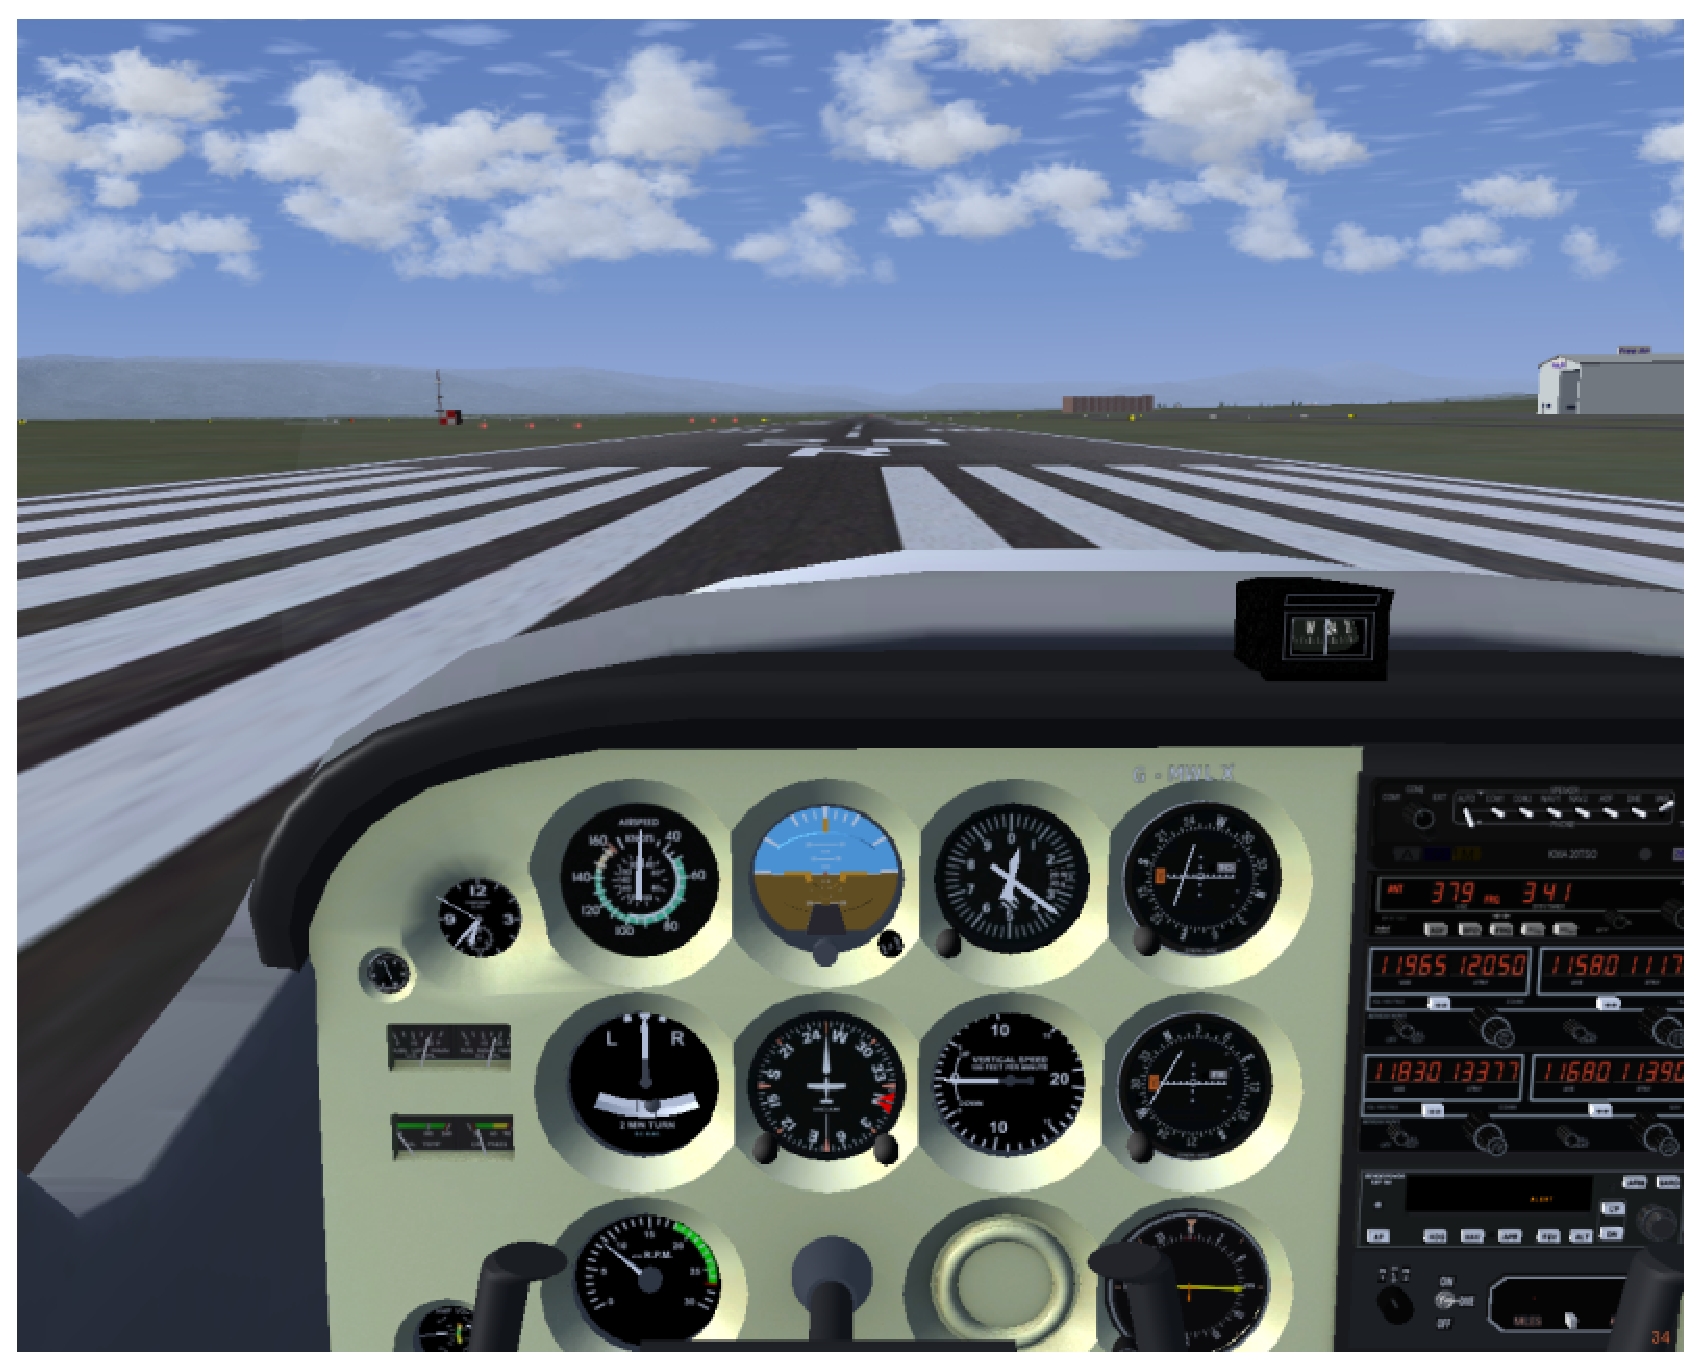
\includegraphics[clip,width=12.5cm]{panel3d}
}}

\smallskip
 \noindent
Fig.\,6: \textit{The 3D cockpit of the Cessna 172.}
\medskip

Aircraft within \FlightGear{} can have both a 2-dimensional instrument panel
and a 3-dimensional cockpit. The 3-dimensional cockpit provides a much
more realistic pilot-eye view, but can be difficult to read with small
monitors.

The default Cessna 172P (c172p) has both a 3-dimensional and 2-dimensional
cockpit. The 3-dimensional cockpit is activated by default when you start
\FlightGear{}, but you can overlay the 2-dimensional instrument panel by
selecting \texttt{View->Toggle 2D Panel} from the menu, or pressing the ``P'' key.

All panel levers and knobs can be operated with the mouse. To change a
control, just click with the left/middle mouse button on the
corresponding knob/lever. For controls that have a range of positions,
using the middle mouse button for larger adjustments. In general, clicking
on the right side of a control will increase the value, while clicking the left side
of the control will decrease the value.

Some instruments (particularly radios) also support use of a mouse scroll-wheel
to change values.

%%%%%%%%%%%%%%%%%%%%%%%%%%%%%%%%%%%%%%%%%%%%%%%%%%%%%%%%%%%%%%%%%%%%%%%%%%%%%%%%
%%%%%%%%%%%%%%%
\section{The Head Up Display\index{head up display}}
%%%%%%%%%%%%%%%%%%%%%%%%%%%%%%%%%%%%%%%%%%%%%%%%%%%%%%%%%%%%%%%%%%%%%%%%%%%%%%%%
%%%%%%%%%%%%%%%

\FlightGear{} also provides a \Index{HUD} (\textbf{H}ead \textbf{U}p
\textbf{D}isplay) \index{head up display}. HUDs are generally found in military
aircraft and some very advanced jets. However, \FlightGear{} also allows you
to use a HUD on many GA aircraft. To activat the HUD, press `h'.

The \Index{HUD} shown in Fig.\,7  displays all main flight parameters of the
plane. In the center you find the \Index{pitch indicator} (in degrees) with the
\Index{aileron indicator} above and the \Index{rudder indicator} below. A
corresponding scale for the elevator\index{elevation indicator} can be found
to the left of the pitch scale along with a pitch trim indicator. On the bottom
there is a simple \Index{turn indicator}.

There are two scales at the extreme left: The inner one displays the \Index{speed}
 (in kts) while the outer one indicates position of the \Index{throttle}.
The two scales on the extreme right display your \Index{height} - the left one
shows the height above ground while the right of it displays hieght above sea-level,
both being displayed in feet.

Besides this, the \Index{HUD} delivers some additions information. On the upper
left you will find date and time, along with your current position, in \Index{latitude}
and \Index{longitude}. 

You can change color of the \textbf{HUD} using the ``H'' or ``'h''  key.
Pressing the toggle ``i/I'' minimizes/maximizes the HUD.

\medskip

 \centerline{\fbox{
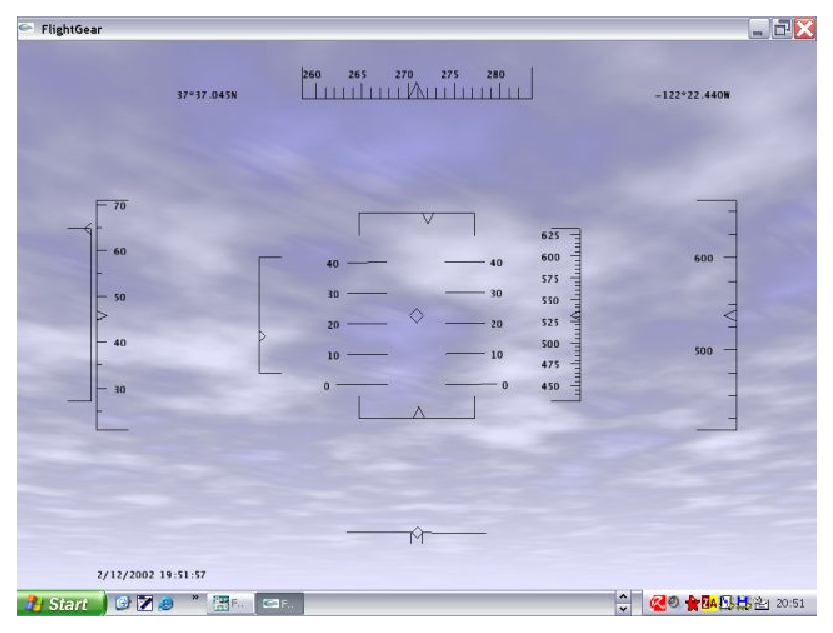
\includegraphics[clip,width=12.5cm]{hud2}
}}

\smallskip
 \noindent
Fig.\,7: \textit{The HUD, or Head Up Display.}
\medskip

%% Revision 0.00  1998/09/08  michael
%% Initial revision for version 0.53.
%% Revision 0.01  1998/09/20  michael
%% several extensions and corrections, added Fig.1.
%% revision 0.10  1998/10/01  michael
%% final proofreading for release
%% revision 0.11  1998/11/01  michael
%% Complete revision of keyborad controls, interesting places
%% revision 0.12  1999/03/07  michael
%% Corrected rudder key
%% revision 0.20  1999/06/04  michael
%% HUD completely rewritten, added panel section with picture, and menu section
%% updated keystrokes
%% revision 0.3 2000/04/20 michael
%% again updated and added keystrokes
%% revised menu entries
%% picture of new panel and re-written panel section
%% added mouse control section
%% Updated many keys, notably autopilot related, added two new tables
%% revision 0.4 2001/05/12 michael
%% updated/added many keystrikes, updated/added panel description
%% (radio stack etc.), new panel pic, panel before HUD now
%% short description of VOR/NDB
%% revision 0.41 2001/01/01 michael
%% added section on flight school material
%% added hints to user configurable *.xml files
%% revision 0.5 2002/01/01 michael
%% revised all changed keybindings now mostly read off of keyboard.xml
%% restructured tables more logically and put into separate files
%% for inclusion in Short Reference
%% New panel picture and revised descirption of panel according to new features
%% New HUD picture
%% revision 0.6 2002/09/05 michael
%% Several corrections/tweaks in plus renumbering of tables
%% Tweaks in menu entries
%% Added 3D cockpit picture
%% Changing numbers in radios
%% Added new menu items, swapped over 3D and 2-D pictures, as 3D cockpit is
%%  now the default
%% Revision 18/10/08: Numerous changes to improve readability, correct spelling errors etc.
%% Revision 8/3/09: Improved description of mouse modes.
%% Revision 26/12/09: Re-organization, move panel description to tutorial, update menu items.

